\subsection{Accuracy of Revision Forecasts}
In the subsequent analysis, we evaluate forecasting performance using the Weighted Interval Score (WIS). To reiterate, the WIS measures the distance between the forecast distribution and the observed target value on the log scale. The quantity \( \exp(\text{WIS}) - 1 \) provides an interpretable approximation of the absolute relative error. The arithmetic mean of WIS captures relative error in log space, which is equivalent to the geometric mean in the original scale. 

The forecasting performance is evaluated relative to a baseline model, defined as a flat-line predictor whose forecasted median is the 7-day moving average of the most recent observations. Consequently, the WIS for the baseline reduces to the absolute error on the log scale between the most recent observation and the finalized.

We evaluate the forecasting performance of our framework across the three datasets described in Section 4.1. For the MA-DPH confirmed cases, which are usually normalized by a constant (the MA population), we generate forecasts only for the counts. For the insurance claims, we produce forecasts for both the counts and the fractions of COVID-19–related outpatient claims. For the antigen tests, we forecast the fraction of positive tests among all tests conducted.


The following is a summary of the experimental results:
\begin{itemize}
    \item Our data revision forecasting framework substantially reduces forecast error, particularly at shorter lags (e.g., within the first 0–5 days). However, the marginal improvement diminishes as the lag increases. These results suggest that modeling and forecasting data revisions is most beneficial in settings where timely estimates are needed in near real-time.
    \item Comparing across the three datasets, we find that the task is most difficult for the insurance claims data, followed by antigent tests, and finally MA-DPH confirmed cases. Intuitively, this ordering matches Figure 1, where the claims data exhibit the slowest convergence among the three.
    \item Abrupt distributional shifts remain a significant challenge. Our model relies on historical data revision patterns to forecast future updates, which implicitly assumes that these patterns are stationary over time. When the revision process undergoes a sudden and substantial change—particularly one that has not been observed in the training data—the model may struggle to adapt, resulting in degraded forecasting performance. 

\end{itemize}

Next, we demonstrate the forecasting performance of our model and how the performance varies along difference dimensions. 

\begin{figure}[h!]
    \centering
    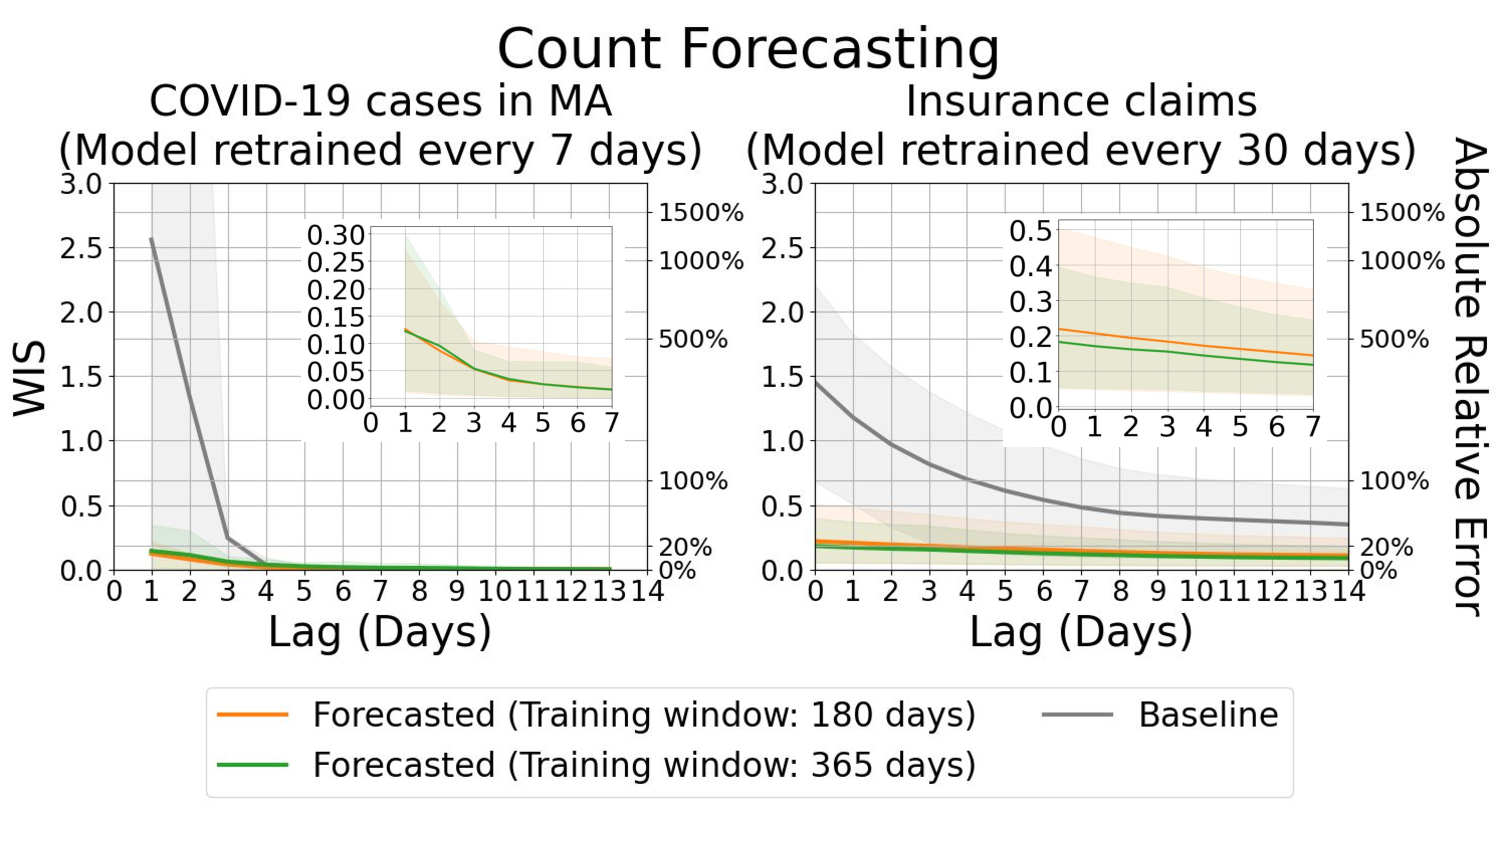
\includegraphics[width=\textwidth]{figs/experiment_count_result_evl_general.pdf}
    \caption{\emph{\textbf{Evaluation of forecasts for counts, aggregated by lag.} Left: Forecasts of finalized confirmed COVID-19 case counts in MA. Right: Forecasts of COVID-19 insurance claims across all states, based on CHNG outpatient insurance claims data. Solid lines indicate the mean WIS, which approximates absolute relative errors between the most recent report and the target, averaged over locations and reference dates for each lag. Shaded areas represent the 10th to 90th percentile interval.}}
\end{figure}

\begin{figure}[h!]
    \centering
    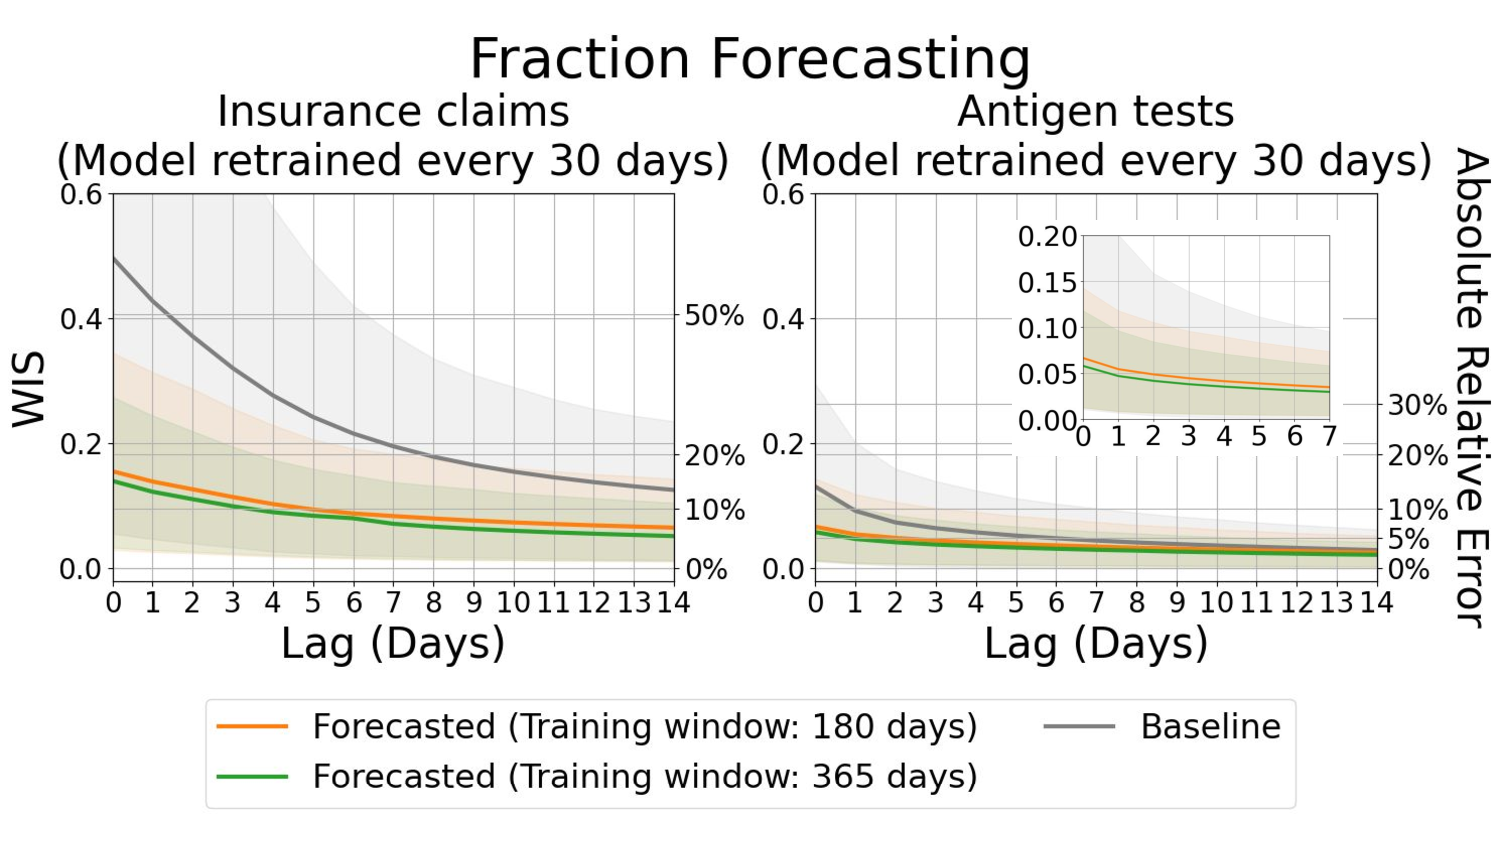
\includegraphics[width=\textwidth]{figs/experiment_fraction_result_evl_general.pdf}
    \caption{\emph{\textbf{Evaluation of forecasts for fractions, aggregated by lag.} Left: Forecasts of the fraction of COVID-19 insurance claims based on CHNG outpatient insurance claims data. Right: Forecasts of the fraction of positive COVID-19 antigen tests based on Quidel antigen tests data. Solid lines represent the mean WIS, , which approximates absolute relative errors between the most recent report and the target, averaged over locations and reference dates for each lag. Shaded areas indicate the 10th to 90th percentile interval.}}
\end{figure}

\subsection{Aggregate Accuracy by Lag}
We investigate how forecasting performance varies as a function of the lag at which the report (or the revision) is made. For a given report date \( s \), we define the forecasting task as having a lag of \( s - t \) when predicting \( Y_{itL} \) using all data available up to and including date \( s \). Since the revision sequence of \( Y_{it} \) gradually converges to its finalized value, forecasts made with shorter lags are inherently more challenging due to the limited availability of information in earlier stages.

Figure 3 and Figure 4 present the evaluation results for count and fraction forecasts, respectively, stratified by lag and averaged over all locations and reference dates. For confirmed cases from MA-DPH (Figure3, left panel), the mean WIS of the baseline model begins at approximately 2.56 when the lag is 1, corresponding to a mean absolute relative error of roughly 1189.43\% under this evaluation metric. In contrast, the mean WIS of our distributional forecasts is substantially lower—0.12 (approximately 13.04\% absolute relative error) when using a 180-day training window, and 0.14 (approximately 15.55\%) when using a 365-day training window. These results demonstrate that our approach outperforms the baseline, particularly when the lag is less than 4 days.

The performance gap is even more pronounced for the insurance claims data, where revision patterns tend to be more frequent and variable. As shown in the right panel of Figure 3, the baseline model maintains a mean WIS above 0.18—corresponding to an absolute relative error of approximately 20\%—even after 14 days of revision. In comparison, our model yields a mean WIS of 0.23 (approximately 25.65\% absolute relative error) at lag 0 (i.e., the first data release) when using a 180-day training window, and 0.20 (approximately 22.65\%) with a 365-day training window. After 14 days of revision, the forecasting accuracy improves with our model achieving a mean WIS of 0.12 (approximately 12.70\% absolute relative error) using the 180-day window, and 0.10 (approximately 10.80\% absolute relative error) using the 365-day window.

Similarly, Figure 4 illustrates the evaluation results of COVID-19 fraction forecasts as a function of lag. For insurance claims data, the mean WIS exceeds 0.45 which approximates an absolute relative error of around 56.83\% when comparing the first release (lag = 0) to the target (lag = 60). However, this mean WIS is reduced to around 0.16  (approximately 16.79\% absolute relative error) using our distributional forecasts with a 180-day training window and a mena WIS of 0.14 (approximately 15.00\% absolute relative error) with a 365-day training window. Even after 7 days of revisions, the distributional forsecasts continue to yield substantial improvements. 

In contrast, the antigen tests are considerably less affected by the data revision problem. Nevertheless, even when provisional reports closely approximate the target, our framework still achieves substantial improvements in forecast accuracy. Specifically, at the first release (lag = 0), the mean WIS decreases from approximately 0.13 (corresponding to a 13.95\% absolute relative error) to 0.07 (6.88\% absolute relative error) when using a 180-day training window, and further to 0.06 (5.97\% absolute relative error) when using a 365-day training window.

\subsection{Aggregate Accuracy by Reference Date}

\begin{figure}[h!]
    \centering
    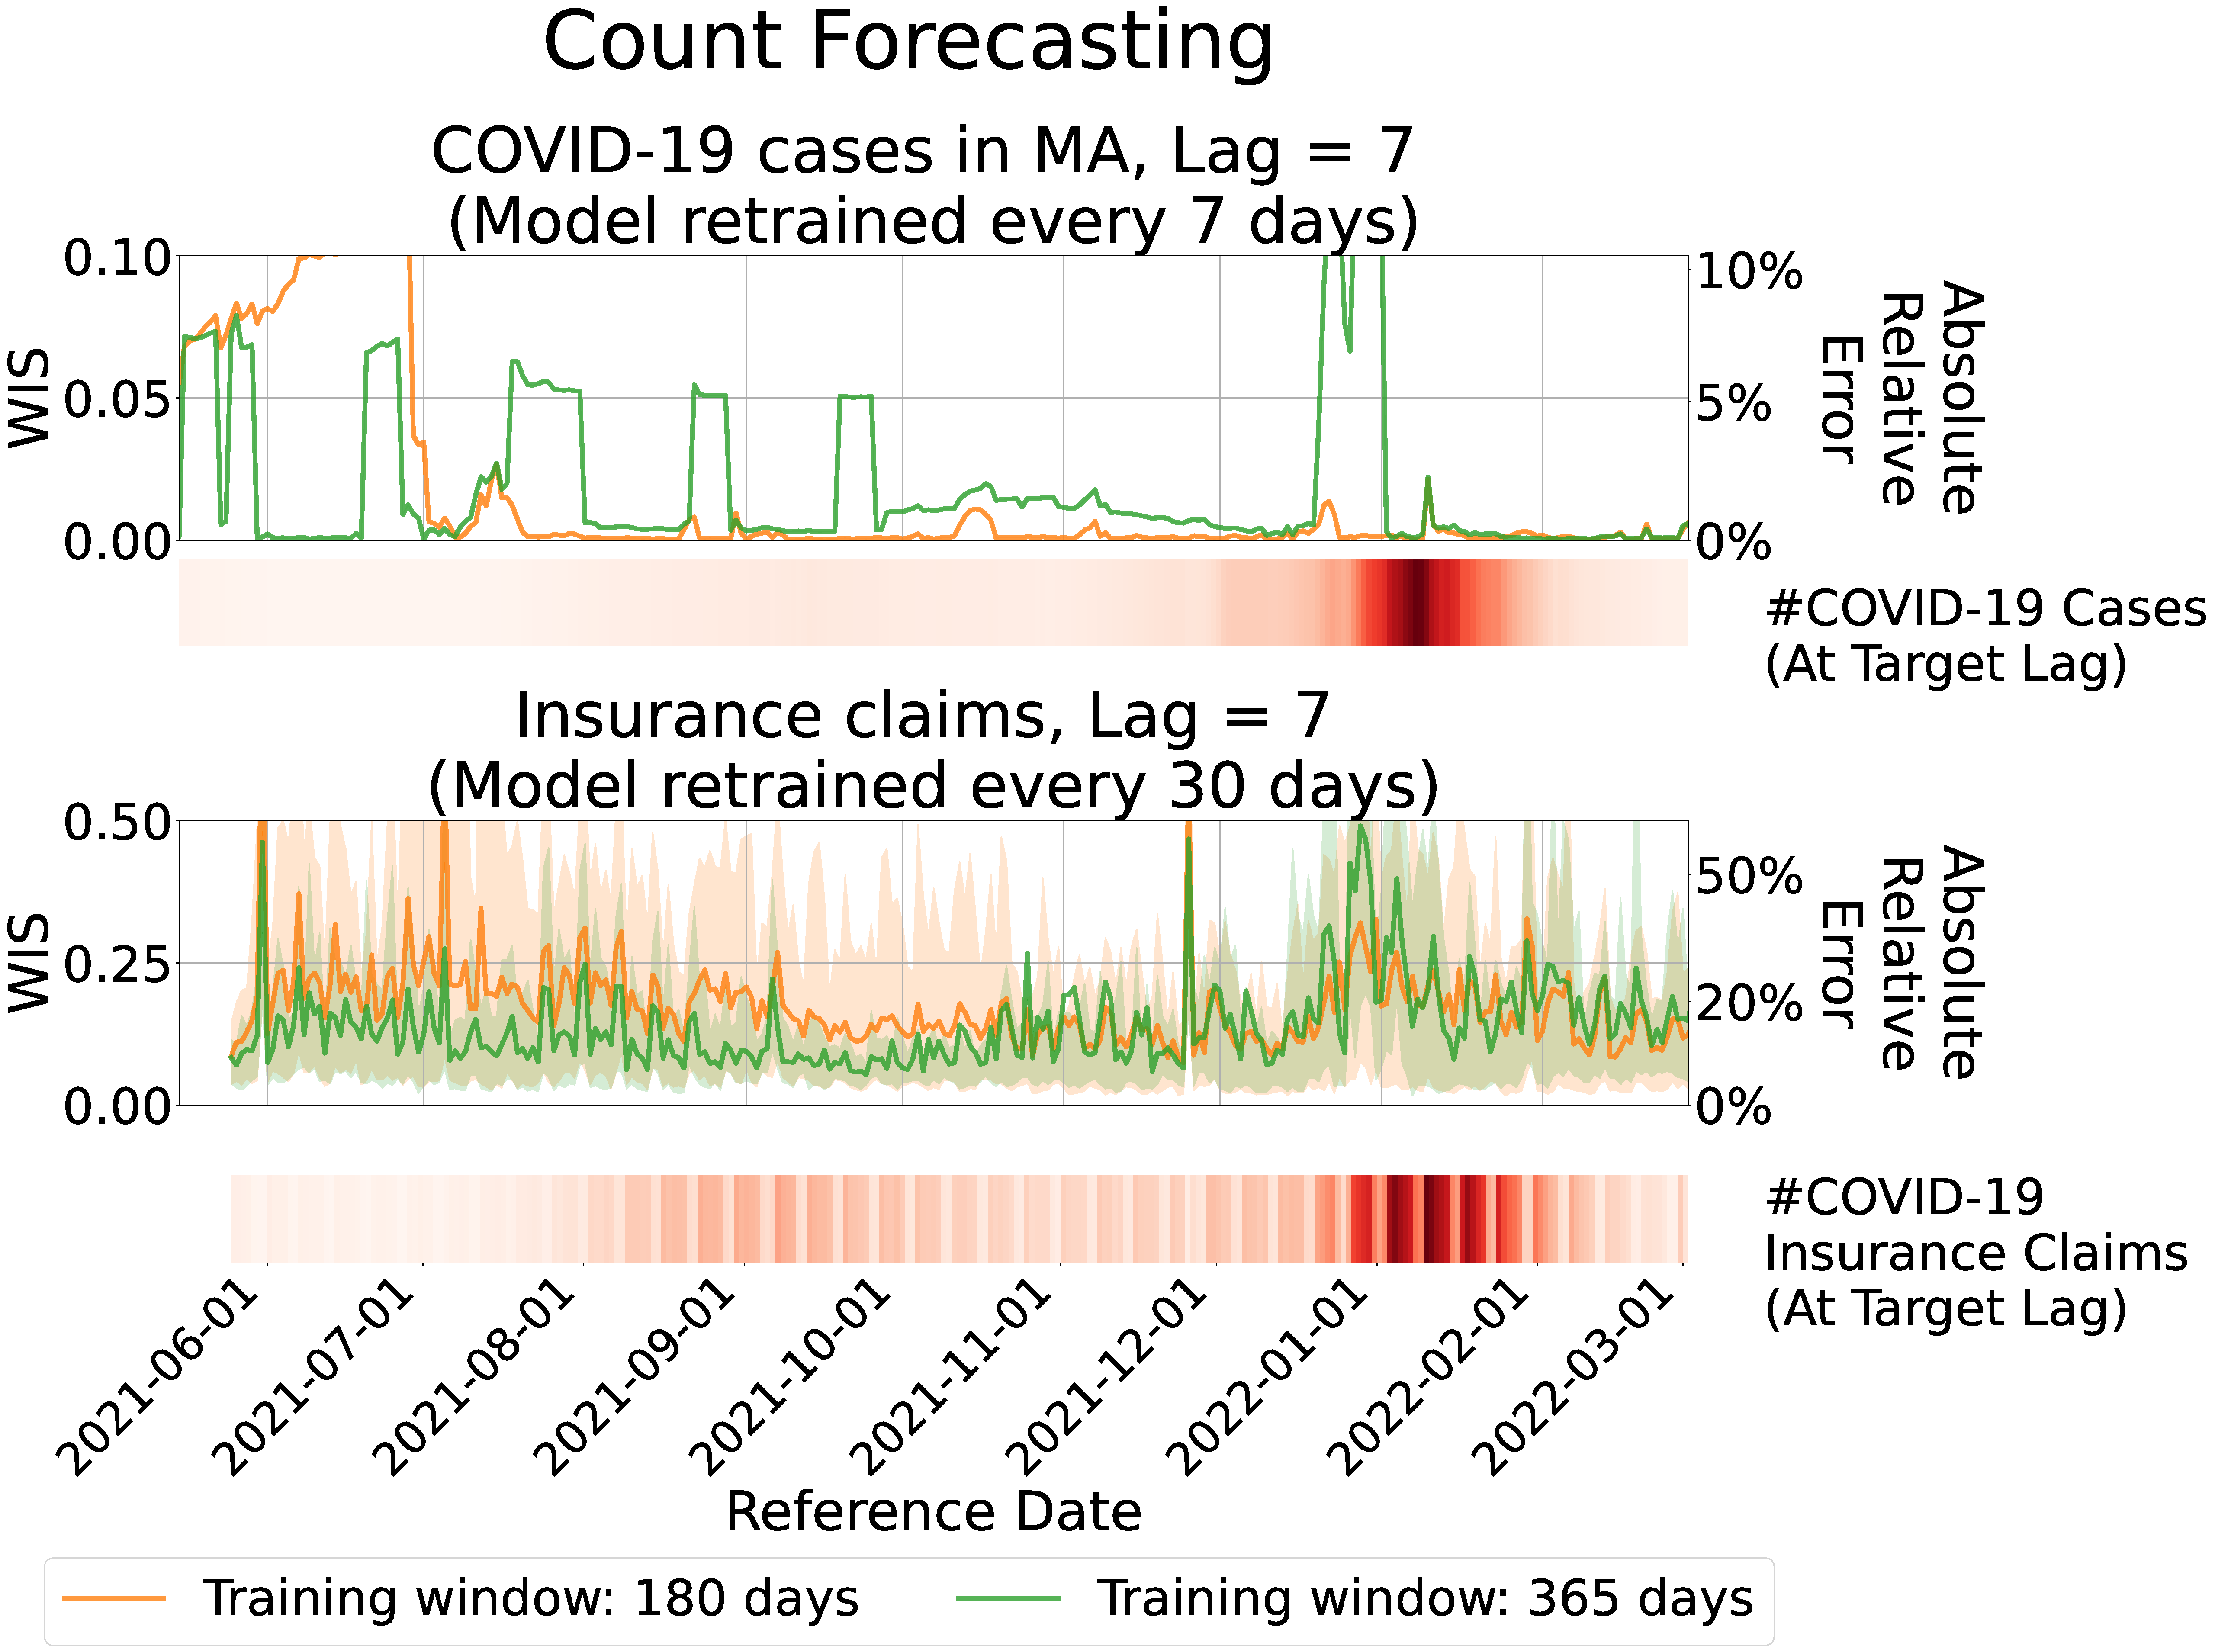
\includegraphics[width=\textwidth]{figs/experiment_count_result_time_series.pdf}
    \caption{\emph{\textbf{Evaluation of forecasts for counts, aggregated by reference date} Top: Forecasts of finalized confirmed COVID-19 case counts in MA. Bottom: Forecasts of COVID-19 insurance claims across all states, based on CHNG outpatient insurance claims data. Solid lines represent the mean WIS at lag 7, averaged over locations for each reference date. Shaded areas indicate the 10th to 90th percentile interval. The accompanying heatmaps display the corresponding target values, with darker shades indicating larger number of cases or claim counts.}}
\end{figure}

\begin{figure}[h!]
    \centering
    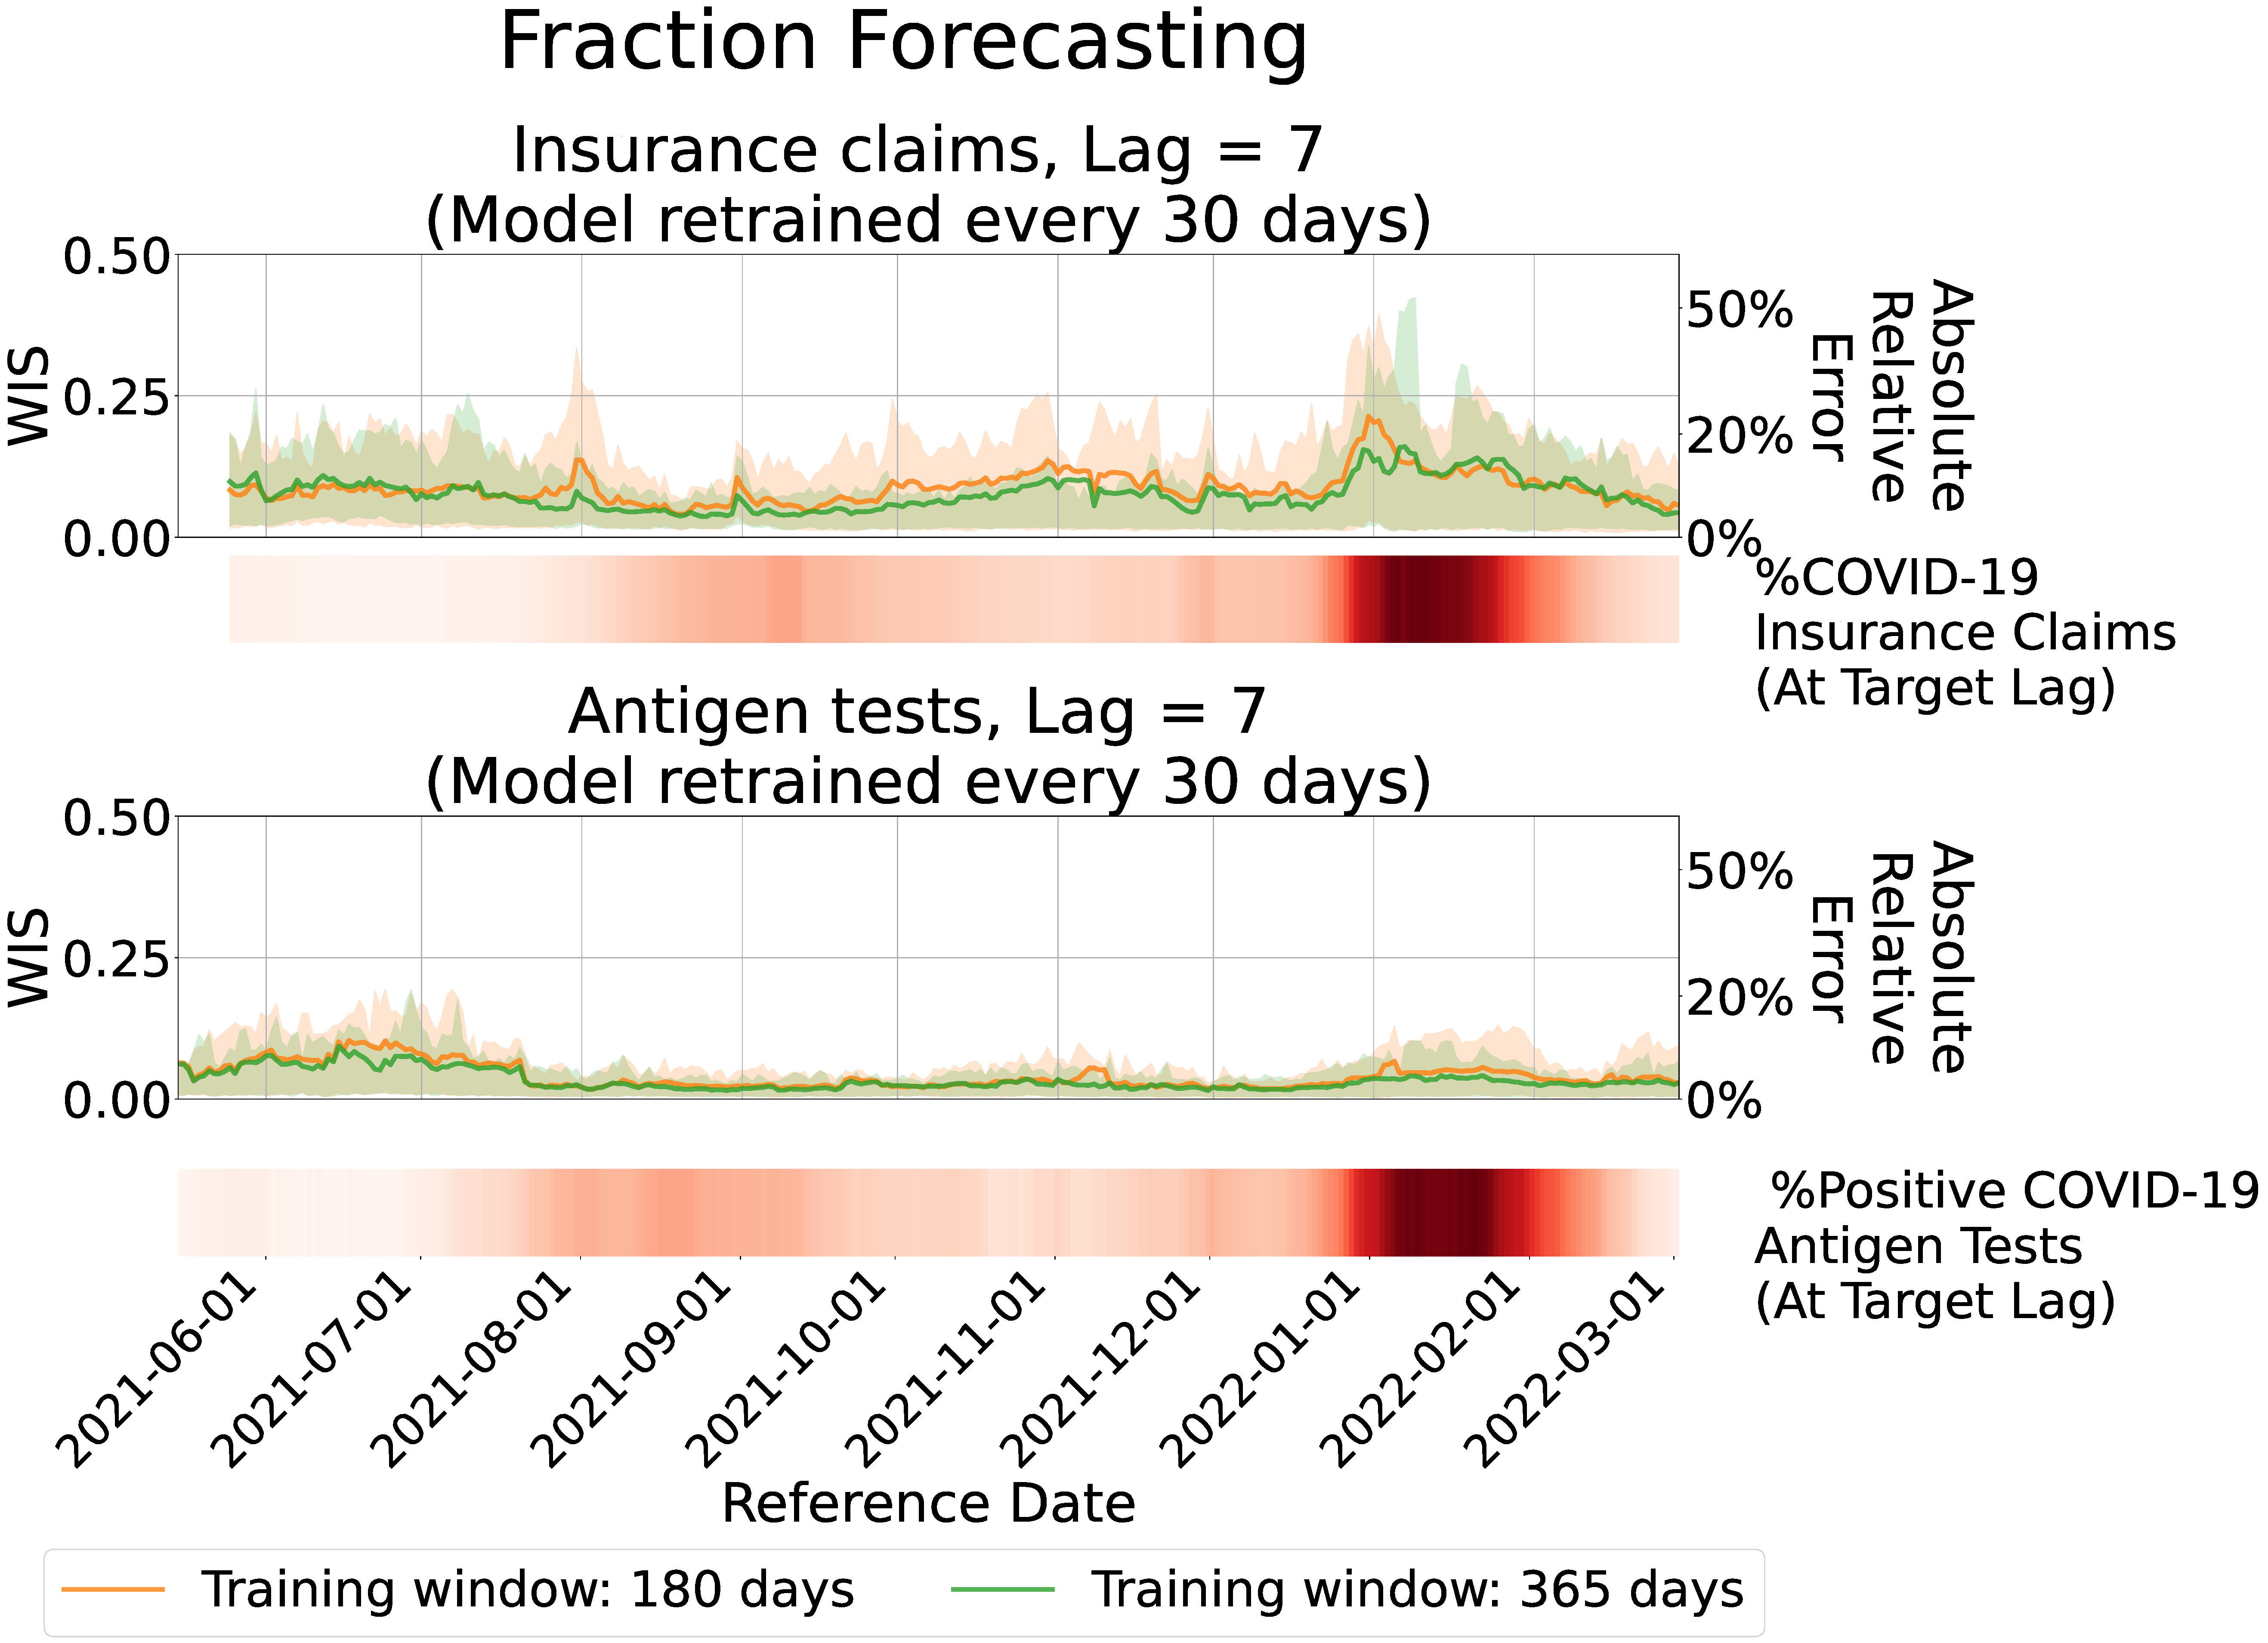
\includegraphics[width=\textwidth]{figs/experiment_fraction_result_time_series.pdf}
    \caption{\emph{\textbf{Evaluation of forecasts for fractions, aggregated by reference date.} Top: Forecasts of the fraction of COVID-19 insurance claims based on CHNG outpatient insurance claims data. Bottom: Forecasts of the fraction of positive COVID-19 antigen tests based on Quidel antigen tests data. Solid lines represent the mean WIS at lag 7, averaged over locations for each reference date. Shaded areas indicate the 10th to 90th percentile interval. The accompanying heatmaps display the target values, with darker shades indicating higher fractions.}}
\end{figure}

The difficulty of the forecasting task varies not only with lag but also over time. Figure 5 and Figure 6 present evaluation results for forecasts made for reference dates from 2021-06-01 to 2022-03-01 at a fixed lag of 7 days, corresponding to count and fraction targets, respectively. The results are stratified by reference date and averaged across all locations. In each figure, the color strip (i.e., a one-dimensional heatmap below the line plot) indicates the target values over time.

Our model generally performs well. A comprehensive set of time series forecast evaluation results for all 50 states is provided in Appendix C. However, the forecast accuracy occasionally declines during periods of rapid epidemiological change, particularly during the Omicron wave (November 2021 to February 2022). This degradation is primarily due to the lagged nature of the model: coefficients estimated from data observed \( L \) days earlier may not adequately capture abrupt shifts in revision patterns, resulting in reduced performance under non-stationary conditions.

The Omicron wave, the largest observed during the COVID-19 pandemic, was characterized by unprecedented infection rates and severe strain on public health reporting systems. In contrast to the preceding Delta wave (July to November 2021), the Omicron surge induced abrupt and substantial changes in the data revision pattern. These shifts posed a significant challenge for our model, which struggled to adapt to revision dynamics not previously encountered in the training data.

Another challenging period is from June to July 2021, characterized by an extremely low general infection rate. Recall that the WIS consists of absolute deviations between the forecasts and the target. This evaluation metric will exaggerate relative errors when the target is extremely small.


\subsection{Impact Factors of Forecast Accuracy}
Our method exhibits degraded performance under two specific scenarios: (1) periods marked by abrupt changes in the target surveillance trend, and (2) periods when the target values are extremely small. The first scenario relates to the direction of the trend in the target surveillance curve, while the second pertains to the magnitude of the target values. We now examine the distribution of WIS across different lags, conditioned separately on each of these two factors, using the CHNG outpatient COVID-19 fraction data as a case study.

The left panel of Figure 7 shows the distribution of WIS across different lags, stratified by the trend direction of the CHNG outpatient COVID-19 fraction. We classify each instance into one of three categories: increasing (“up”), decreasing (“down”), or stable (“flat”) trends. The trend indicator \( Z_{it} \) is defined as:

\[
Z_{it} =
\begin{cases}
    1, & \text{if } \frac{\widetilde{Y}_{itL}}{\widetilde{Y}_{i(t-7)L}} \geq 1.25 \\
    -1, & \text{if } \frac{\widetilde{Y}_{itL}}{\widetilde{Y}_{i(t-7)L}} \leq 0.75 \\
    0, & \text{otherwise}
\end{cases}
\]

We assign \( Z_{it} = 1 \) if the 7-day average of the target value has increased by at least 25\% relative to the previous week, indicating an upward trend for location \( i \) at date \( t \). Conversely, \( Z_{it} = -1 \) denotes a decrease of at least 25\%, indicating a downward trend. All other cases are classified as flat (\( Z_{it} = 0 \)).



\begin{figure}[h!]
    \centering
    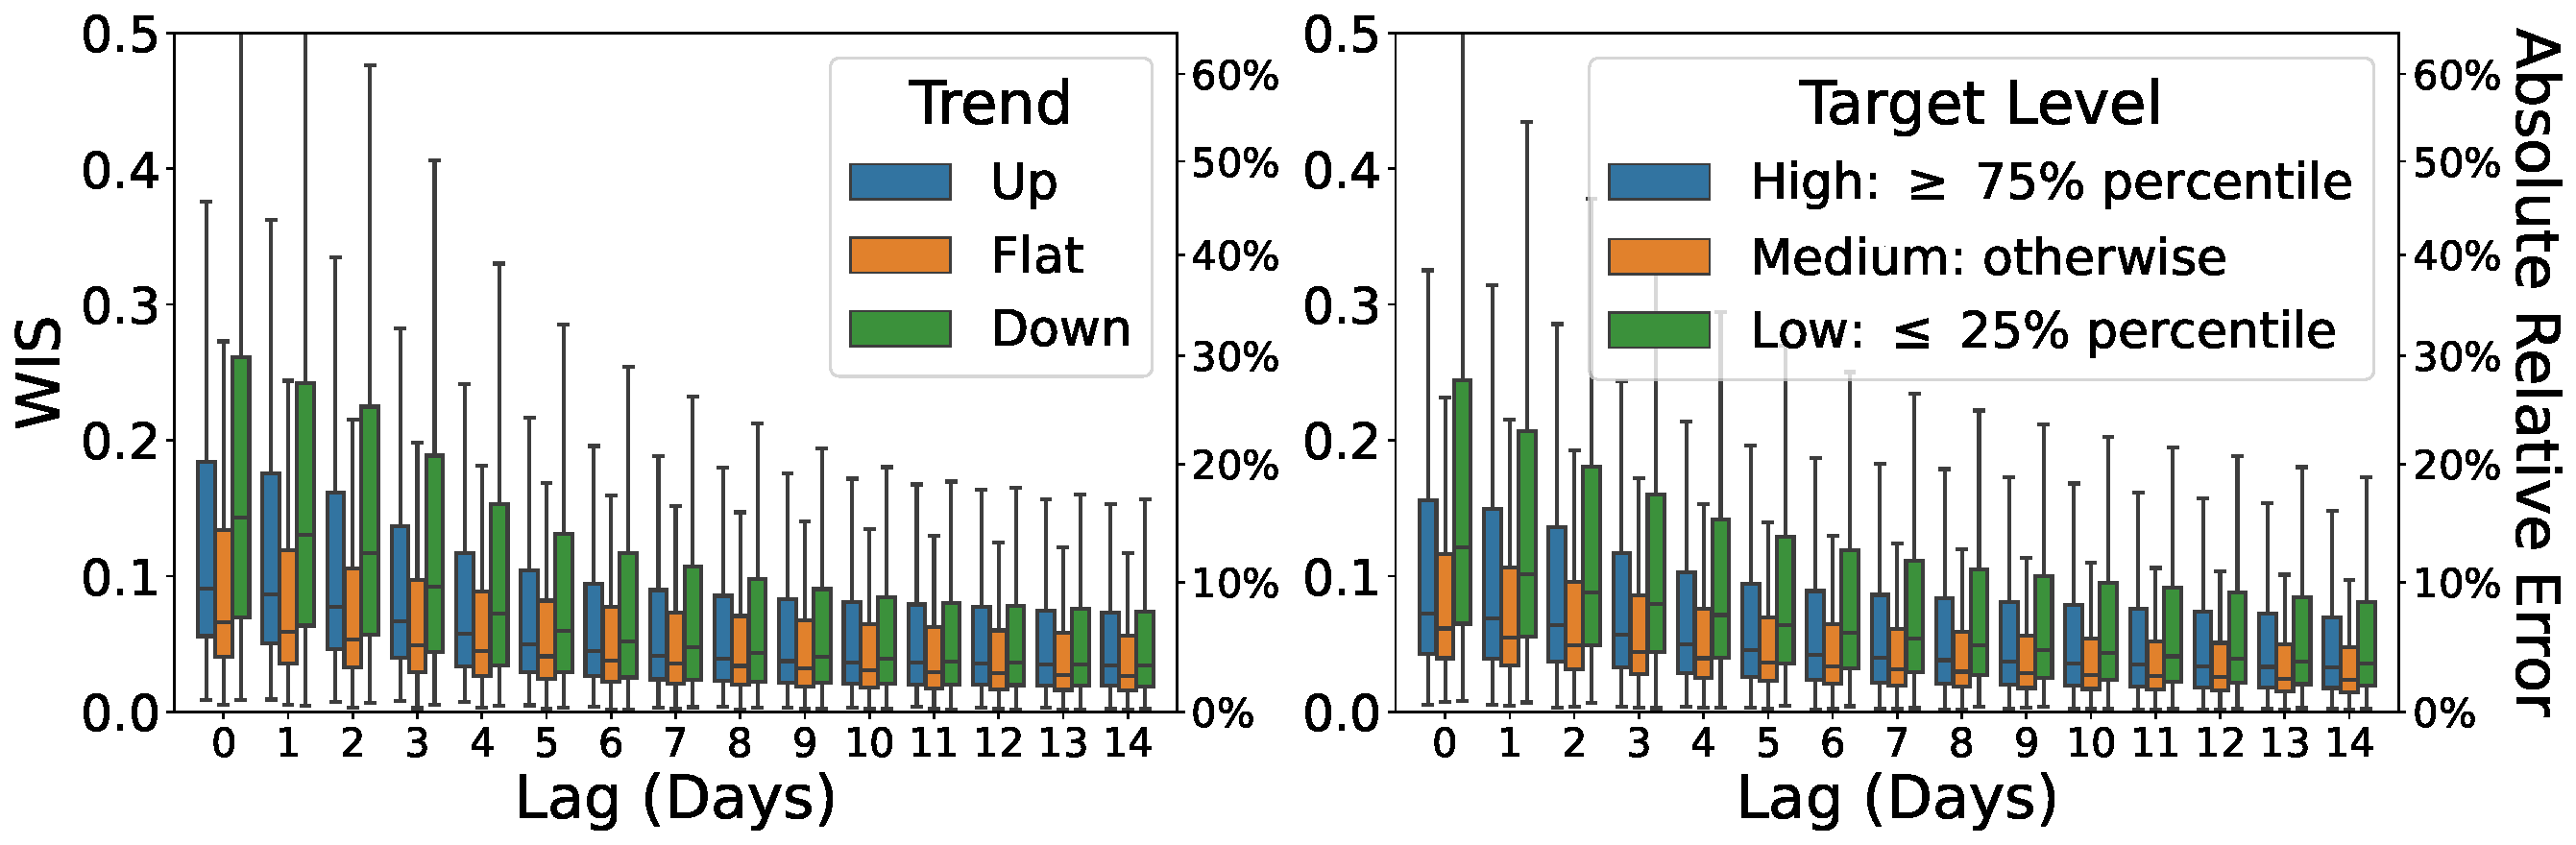
\includegraphics[width=\textwidth]{figs/experiment_fraction_result_factors.pdf}
    \caption{\emph{\textbf{Boxenplots illustrating the impact of surveillance conditions on forecast accuracy} (Each box displays the 25th, 50th (median), and 75th percentiles of the WIS). Left: Forecasts stratified by the direction of the target surveillance trend—"Up", "Flat", or "Down". Right: Forecasts stratified by the magnitude of the target, categorized as "High", "Medium", or "Low".}}
\end{figure}

Forecasting performance notably improves during periods with minimal changes in the target surveillance curve. The performance is the poorest during “Down” periods for quantities with only 0–7 revisions. This can be attributed to the fact that the “Down” category primarily corresponds to the downswing of the Omicron wave, whereas the “Up” category includes reference dates from the upswings of both the Delta and Omicron waves (as shown in Figure S52 in Appendix D). Overall, the model performs better during the Delta wave than during the Omicron wave, as the magnitude of distributional shift in the data revision pattern during Delta was comparatively smaller. After the first 7 revisions, the performance gap across the three trend categories narrows, with the performance ranking shifting to: “Flat”, “Down” and then “Up”.

The right panel of Figure 7 illustrates the distribution of WIS over lags, stratified by whether the target surveillance value falls into the categories of "High", "Medium", or "Low". A target value is classified as "High" if it is greater than or equal to the 75\% percentile, while it is classified as "Low" if it is less than or equal to the 25\% percentile. The performance order, from best to worst, consistently ranks as "Medium", "High", "Low" across lags. Notably, even after the first 14 revisions, the performance gap across these three categories remains significant.


\subsection{Comparison of Performance with Alternative Methods}
In this section, we demonstrate that our model achieves forecast accuracy comparable to, or exceeding, that of NobBS\cite{McGough2020} and Epinowcast\cite{epinowcast}, while substantially reducing computational runtime. These two methods were selected for comparison as they are among the most established in the literature, widely used in public health research projects, and supported by well-maintained R packages.

Since both methods are specifically designed for count-type data, our comparison is limited to count-type datasets. For the COVID-19 insurance claims with daily observations, we use a 180-day training window and a target lag of 60 days. To ensure a fair comparison, we apply the same 180-day moving window and a maximum delay of 60 days to NobBS and Epinowcast. To manage computational demands while maintaining consistency across models, we train all methods—including Delphi-RF—at 30-day intervals. Additionally, we evaluate performance on daily confirmed cases from MA-DPH, where revisions stabilize more quickly. For this dataset, we adjust the training frequency to every 7 days, set the maximum delay to 14 days, and maintain the 180-day moving window. In Delphi-RF, the target lag is also set to 14 days to align with these adjustments.

We further extend our comparison to weekly data. To ensure compatibility with weekly data, covariates containing daily change information were excluded. The full model is expressed as:

\begin{align*} 
&Q_{f(Y_{itL}))|X_{itl}}^{\tau} \\
=  &X_{itl}\beta^{\tau}\\
 = &\beta_0^{\tau}  + \mathbf{I}_{\text{first-week}(t+l)}\beta_{1}^{\tau} &&(\text{Intercept, week-of-month effects})\\ 
& + f(Y_{itl})\beta_{2}^{\tau} + \mathbf{e}_{\sqrt{Y_{itl}}}\beta_{3:5}^{\tau} &&(\text{Disease activity level}) \\ 
&+ \left(f(Y_{i(t-7)(l+7)}) - f(Y_{i(t-7)l_{\text{min}}})\right) \beta_{6}^{\tau}
&& \text{(Recent revision magnitude, \(t{-}7\))} \\
&+ \left(f(Y_{i(t-14)(l+14)}) - f(Y_{i(t-14)l_{\text{min}}})\right) \beta_{7}^{\tau}
&& \text{(Recent revision magnitude, \(t{-}14\))} \\
& + f(Y_{i(t-7)(l+7)}) \beta_{8}^{\tau} + f(Y_{i(t-14)(l+14)}) \beta_{9}^{\tau}
&& \text{(Short-term epidemic trends)}\\
\end{align*}

where \(Y_{itl}\) represents the counts reported for the week spanning reference dates \(t-6\) to \(t\), as of the report date \(t+l\), for location \(i\). 

To further evaluate model performance across diverse surveillance settings, we test the models on two additional datasets with distinct characteristics to assess their robustness. First, we apply the models to Puerto Rico (PR) dengue weekly surveillance data spanning from 1991-12-23 to 2010-11-29 (989 weeks). This dataset features a long historical record and strong seasonality, differs from the more irregular trends observed in COVID-19 data. Applying our method to the dengue data enables assessment of its ability to capture seasonal dynamics and long-term surveillance patterns. The target lag is set to 10 weeks, with 104 weeks of data used for training. For comparison, weekly forecasts are generated using NobBS and Epinowcast over the same time period. The maximum reporting delay is set to 10 weeks, and a 104-week moving window is applied, consistent with the setup in\cite{McGough2020}. For all three models, training and forecasting were conducted on a weekly basis.

We also test the models on national weekly influenza-like illness (ILI) case counts from 2014-06-30 to 2017-09-25 (170 weeks), which follow a distinct reporting pattern. For Delphi-RF, a 27-week training window is used with a target lag of 26 weeks. NobBS and Epinowcast are similarly configured with a 26-week maximum delay and a 27-week moving window, following the same settings in\cite{McGough2020}.


\begin{figure}[h!]
    \centering
    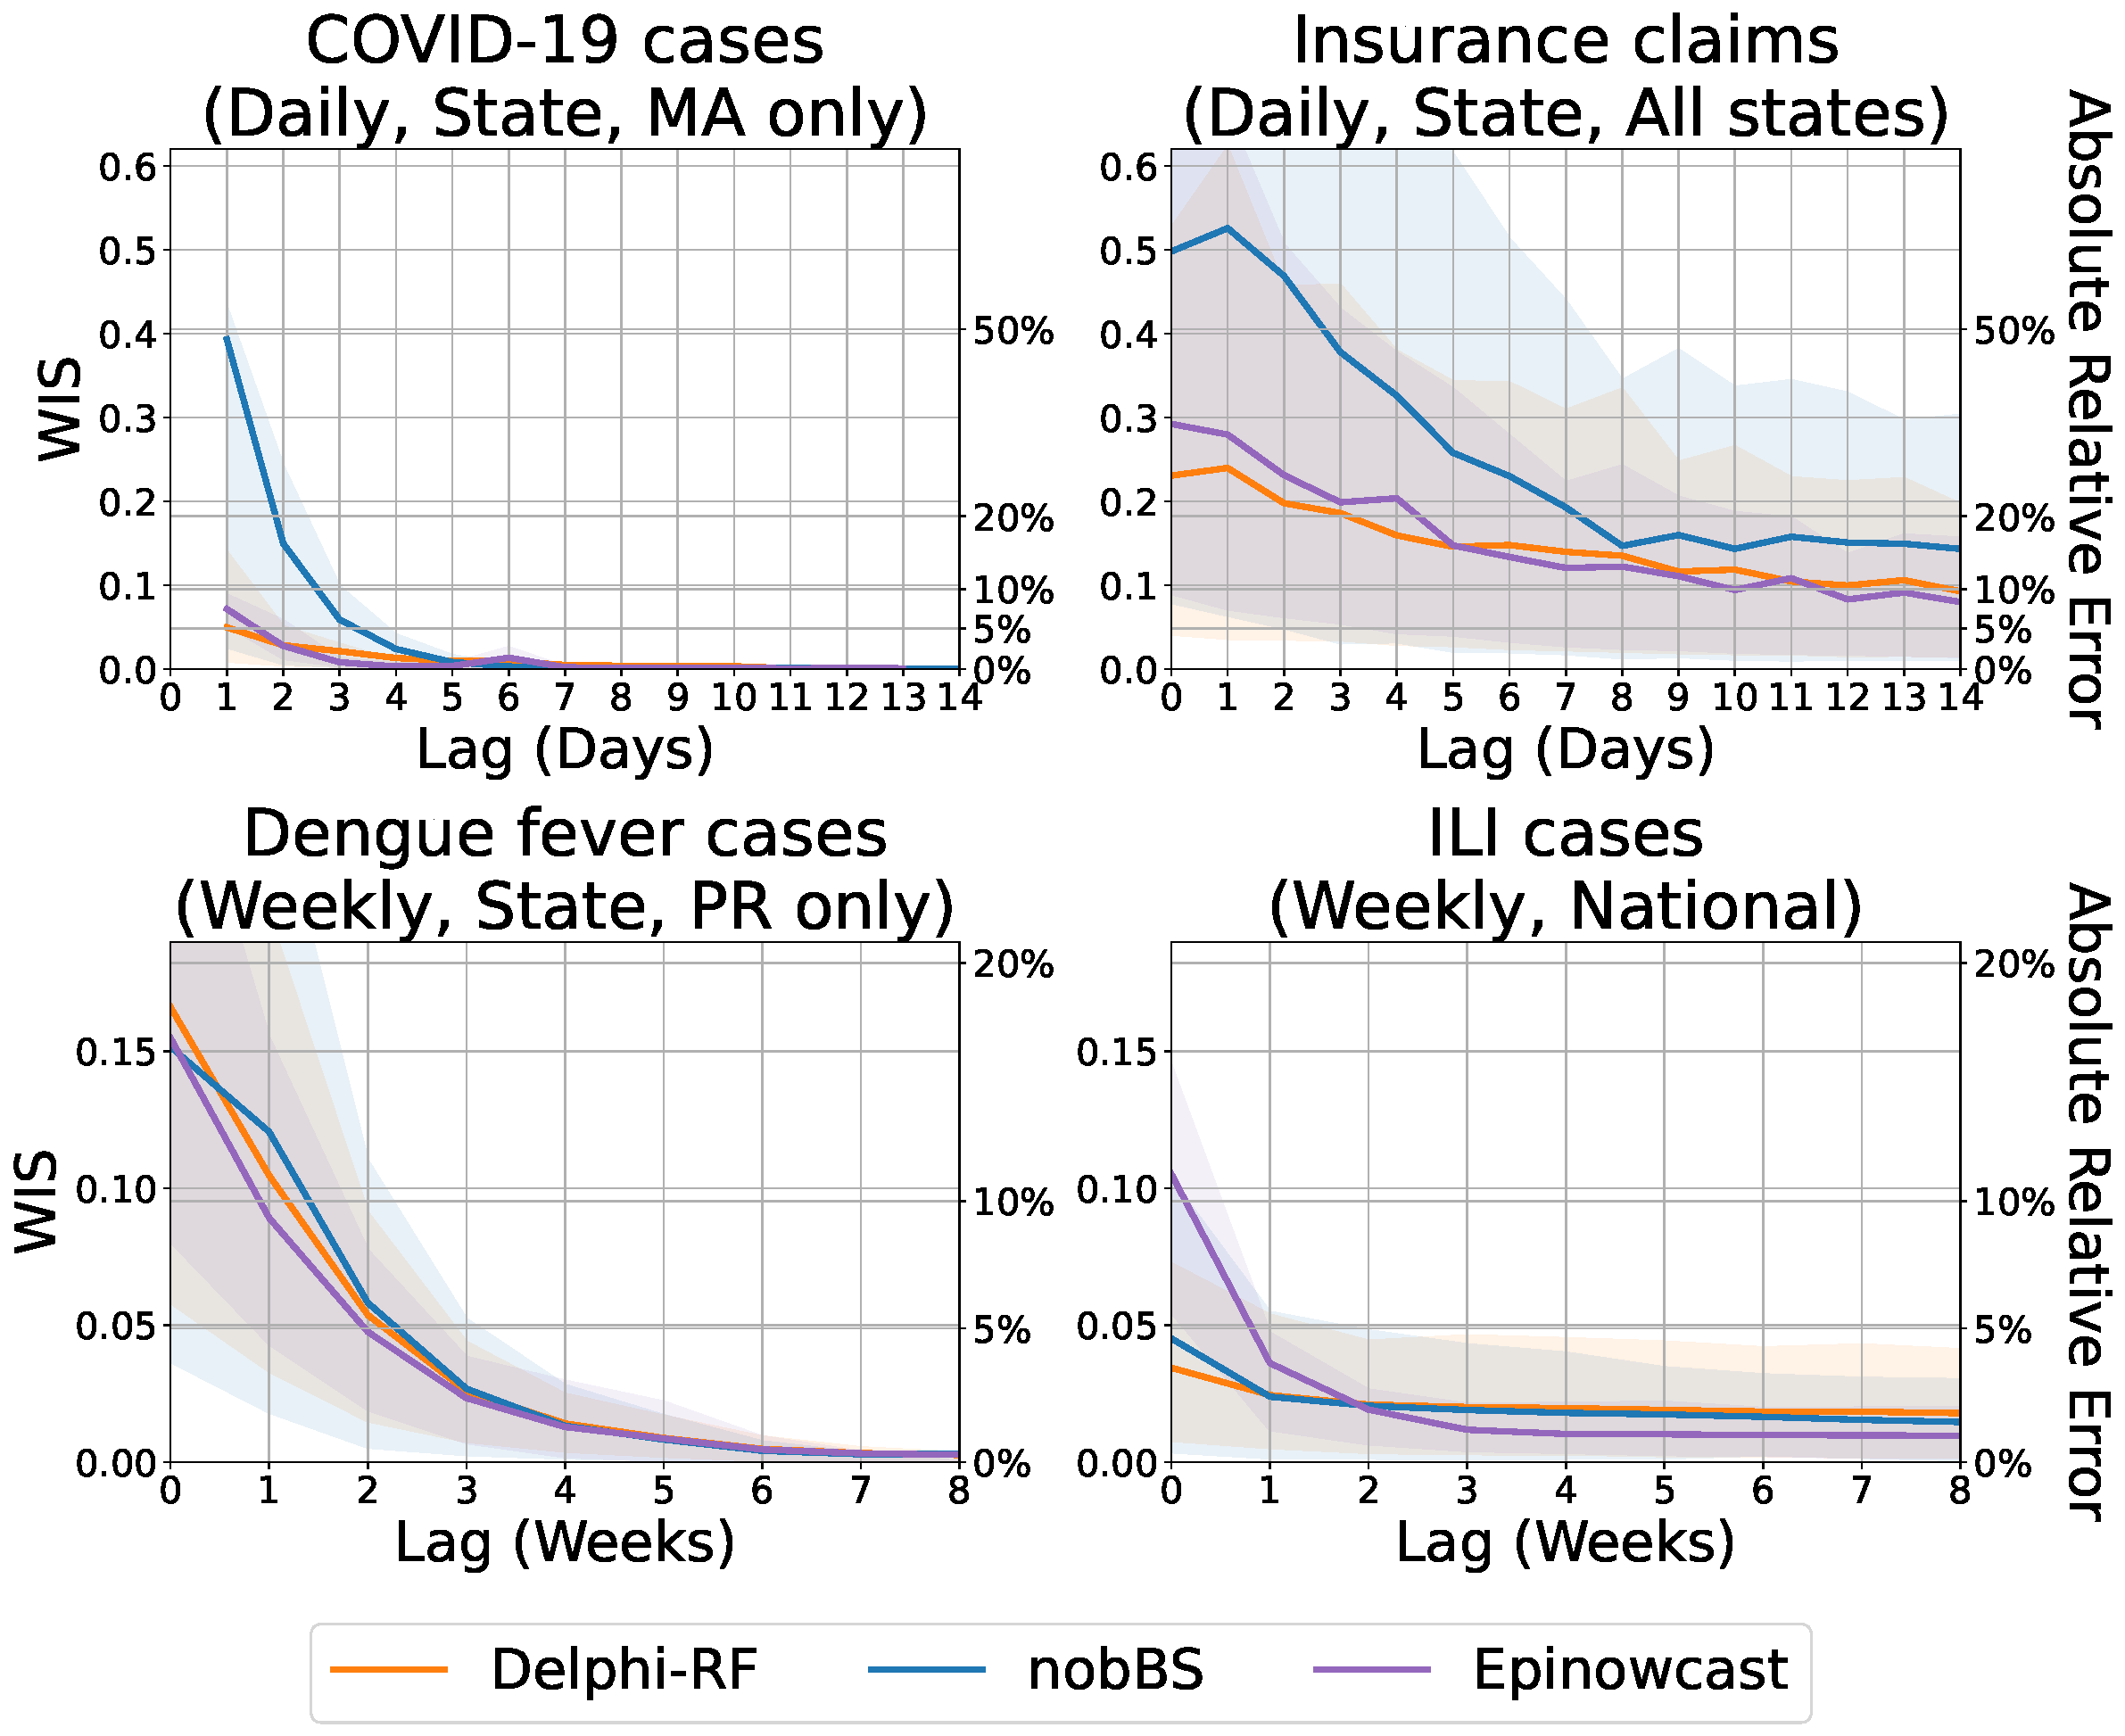
\includegraphics[width=\textwidth]{figs/experiment_count_result_evl_general_for_comparison.pdf}
   \caption{\emph{\textbf{Comparison of count forecast evaluation results with NobBS and Epinowcast.} Top: Forecasts of the number of finalized confirmed COVID-19 case counts in MA and forecasts of the number of insurance claims in all states based on CHNG outpatient insurance claims data. Bottom: Forecasts of the number of dengue fever cases in Puerto Rico and forecasts of the number of ILI case counts nationwide. Solid lines represent the mean WIS, which approximates absolute relative errors between the most recent report and the target, averaged over locations and reference dates for each lag. Shaded areas indicate the 10th to 90th percentile interval.}}

\end{figure}

All experiments were conducted on an Apple Mac Mini equipped with a 3.0 GHz 6-core Intel Core i5 processor, running R version 4.4.2.

\begin{table}[h!]
\centering
\resizebox{\textwidth}{!}{%

\begin{tabular}{cc|cccc}
\hline
\multicolumn{2}{c|}{\multirow{2}{*}{\makecell{\textbf{Computing Time(s)}\\\makecell{(per location\\per report date)\\}}}} 
& \multicolumn{4}{c}{\textbf{Model}} \\
\multicolumn{2}{c|}{} 
& \makecell{Delphi-RF\\Training\\(once/week or month)} 
& \makecell{Delphi-RF\\Testing} 
& \makecell{Epinowcast} 
& \makecell{NobBS} \\
\hline
\multirow{6}{*}{\rotatebox{90}{\textbf{Dataset}}} &\makecell{Confirmed Cases\\(Daily, State, MA only)} & $6.773 \pm 0.018$ &$0.369\pm 0.006$  &$406.097\pm 16.190$ &$24.220\pm 0.675$ \\
&\makecell{Insurance Claims \\ (Daily, State, All states)}   & $23.712\pm 0.029$ &$0.819\pm 0.008$&$2386.512 \pm 230.895$ &$96.012 \pm  0.453$ \\
 
% &\makecell{Insurance Claims\\(Weekly, State)} &$0.408 \pm 0.001$ &$0.003\pm 0.000$ &$10.332 \pm 0.129$ &$1.638 \pm 0.002$ \\ 
 &\makecell{Dengue Fever Cases\\(Weekly, State, PR only)} &$6.848 \pm 0.106$ &$0.153\pm 0.008$  &$64.628 \pm 0.395$ &$8.337\pm 0.033$ \\
 &\makecell{ILI Cases\\(Weekly, National)} &$2.006 \pm  0.032$ &$0.136\pm 0.003$  &$18.373 \pm 2.139$ &$5.960\pm 0.055$ \\
 \hline
\end{tabular}
}
\caption{\emph{\textbf{Computing time comparison across methods and datasets.} 
Computing time required by different methods applied to various datasets, measured per location and per report date. 
The table presents the mean and standard error of the mean (SEM) for computing time. For daily data, all models are trained and generate forecasts every 30 days for CHNG outpatient insurance claims and every 7 days for MA-DPH COVID-19 confirmed cases. For weekly data, models are trained and generate forecasts on a weekly basis. To ensure a fair comparison, all settings—including maximum delay and training window size—are kept the same across methods.}}

\label{tab:full-width}
\end{table}

As shown in Figure 8, our model delivers accurate forecasts across all evaluated datasets. For daily COVID-19 signals, Delphi-RF consistently outperforms NobBS and achieves accuracy comparable to that of Epinowcast. To ensure a fair comparison across methods, a fixed 180-day training window is used—a conservative choice made to accommodate the computational demands of more resource-intensive methods such as Epinowcast. This restriction, however, can be suboptimal for Delphi-RF. In fact, forecast accuracy improves for certain reference dates and locations when the training window is extended (e.g., FL and NJ in Figures S10 and S32, Appendix C), with only a modest increase in computation time. For example, increasing the window to 365 days results in less than a twofold increase in runtime for both the Insurance Claims and MA-DPH COVID-19 case data (Table 2, Appendix B). In contrast, Epinowcast and NobBS become computationally infeasible under the same setting, with Epinowcast exceeding the 30-minute runtime cutoff for a single location–report-date pair. When applied to Insurance Claims data across all 50 states, sequential training using either method with a 180-day or longer window would require more than two days—rendering them impractical for daily forecasting tasks.

For weekly data, Delphi-RF exhibits competitive forecasting performance for dengue fever cases in Puerto Rico. In the case of national ILI counts, Delphi-RF outperforms both benchmark methods at lag 0. Although Delphi-RF does not outperform Epinowcast when the reporting lag exceeds 3 weeks, the absolute relative errors for all methods are sufficiently low—consistently below 2.5\%—rendering performance differences practically negligible.

The runtime reported in Table 1 reflects both the training and testing phases required by our model (including the computing time for data pre-processing), which is substantially faster than the other two methods. Unlike Epinowcast and NobBS, which require simultaneous training and forecasting, our model benefits from the modularity of machine learning frameworks, allowing for independent training and inference. Once trained, the model can be repeatedly applied to generate forecasts for new data. This flexibility allows users to tailor the training frequency to operational constraints, a feature not available in Epinowcast or NobBS. The efficiency also enables our model to produce revision forecasts for multiple signals at different temporal resolutions in real time while requiring significantly fewer computational resources. 






